\section{Demo for LaTeX}

This is a demo.

\subsection{Math mode}

This is a paragraph that includes the math formula $x^2 = \pi$.  Another way to write math is to use it separate as
$$
x_1^{2+a} + \frac{x^2+1}{5} \geq 42
$$
and then we have more text.

\subsection{Multiple lines of equations}

This is another example.
\begin{eqnarray*}
& \min & x + y \\
& \mbox{s.t.} & y \leq 20 \\
& & 4x + 2y \leq 15 \\
& & x,y \geq 0
\end{eqnarray*}

\subsection{Figures}
This is how we insert figures.  Figure \ref{fig:figure1} is an example.

\begin{figure}[htb]
\begin{center}

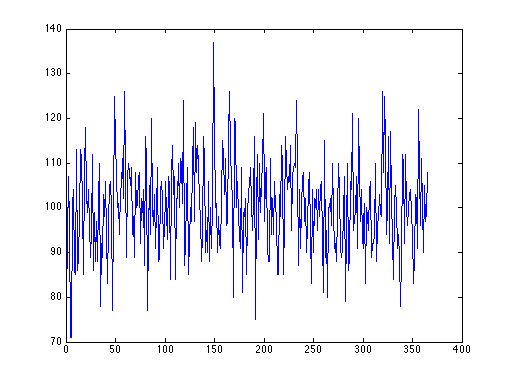
\includegraphics[width=0.75\textwidth]{fig1}
\caption{This is a figure with a caption, here's some math: $x^2$}
\label{fig:figure1}
\end{center}
\end{figure}

And here we have Figure \ref{fig:figure2}.


\begin{figure}
\centering
\begin{subfigure}{.45\textwidth}
  \centering
  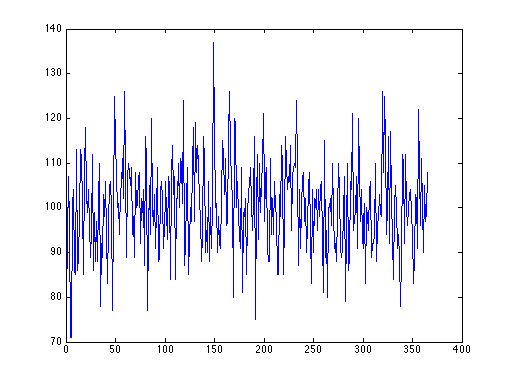
\includegraphics[width=0.95\linewidth]{fig1}
  \caption{A subfigure}
  \label{fig2:sub1}
\end{subfigure}
\begin{subfigure}{.45\textwidth}
  \centering
  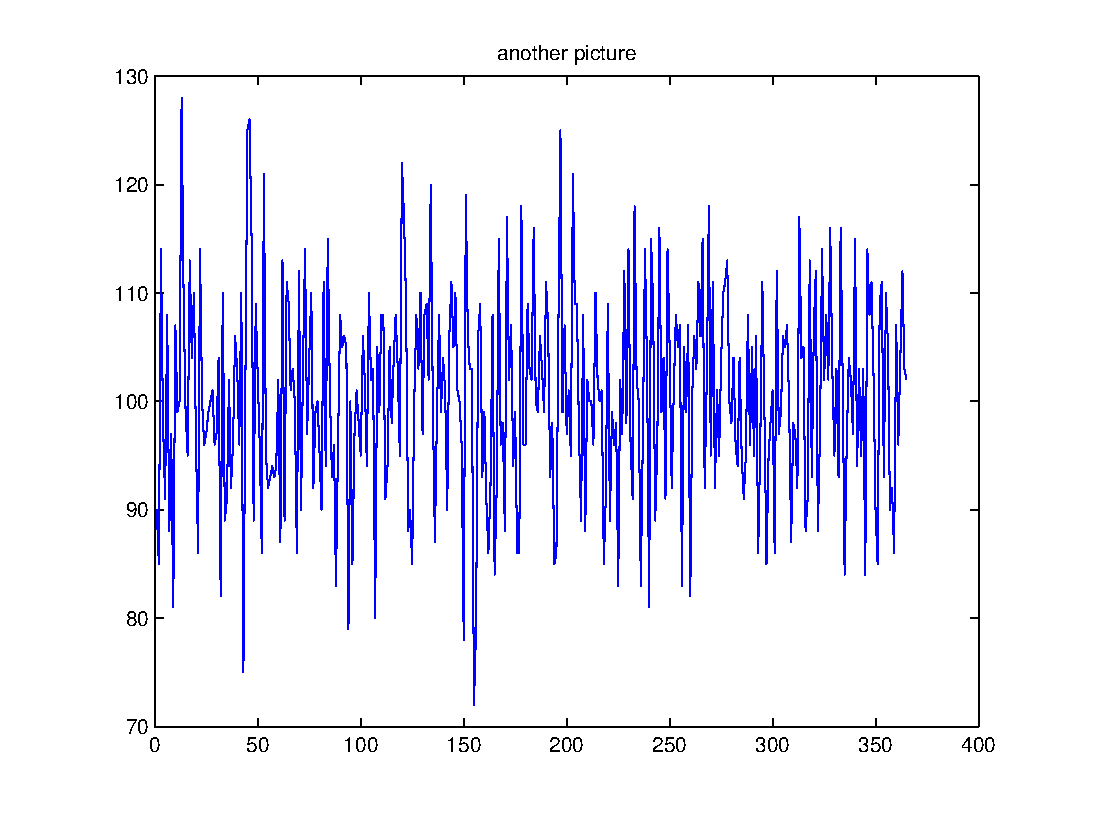
\includegraphics[width=0.95\linewidth]{fig2}
  \caption{Another subfigure}
  \label{fig2:sub2}
\end{subfigure}
\caption{The whole thing...}
\label{fig:figure2}
\end{figure}


\subsection{Tables}

\noindent Tables in LaTeX can be a bit tricky.  Table \ref{tab:table1} shows one example.

\begin{table}
\centering
\caption{Here is some caption}
\label{tab:table1}
\begin{tabular}{c|cccc}
1 & 2 & 3 & 4 & 5 \\
\hline
2 & 3 & 4 & 5 & 6 \\
3 & 4 & 5 & 6 & 7 \\
4 & 5 & 6 & 7 & 8
\end{tabular}
\end{table}



